\chapter{Implementácia}

V rámci riešenia práce sme navrhli aplikáciu na demonštráciu rozšírenej reality obohatenú o oklúziu fyzických objektov.

V tejto kapitole popisujeme proces vývoja demo aplikácie od začiatku po finálnu verziu. Pre takúto demonštráciu je potrebné vyriešiť niekoľko problémov. Získať, alebo vyrobiť samotný oklúder a jeho digitálnu 3D reprezentáciu. Je potrebné vymodelovať objekty, ktoré chceme vykreslovať a naimportovať ich do grafickej knižnice. Tiež potrebujeme nejakým spôsobom registrovať scénu, do ktorej chceme objekty vykresľovať. Potrebujeme nakalibrovať kameru, aby bola ilúzia čo najpresnejšia. Na záver potrebujeme vyriešiť, ako implementovať samotnú oklúziu.

Táto kapitola opisuje všetky kroky schémy znázornenej na obrázku \ref{schema}.

\begin{figure}[h]
 \centering
 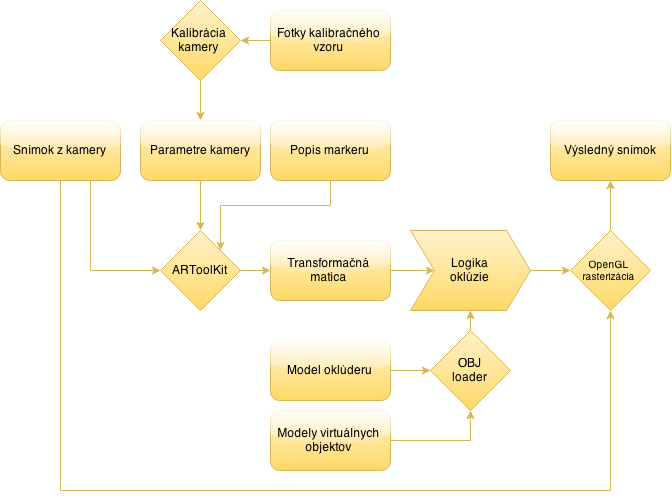
\includegraphics[max width=\textwidth]{pictures/schema.png}
 \caption{Podrobná schéma demo aplikácie}
 \label{schema}
 \end{figure}

\section{Zjednodušená demonštrácia}
\label{section-prototyp}

Na obrázku je snímok obrazovky prvého funkčného prototypu našej demo aplikácie. Aplikácia registruje scénu pomocou markeru a dokresľuje na ňu virtuálnu kocku okludovanú fyzickou kockou. Na obrázku \ref{prototyp} sa nachádza snímok obrazovky tohto skorého prototypu. Kroky tohto procesu sú chronologicky popísané v nasledujúcich sekciách.

\begin{figure}[h]
 \centering
 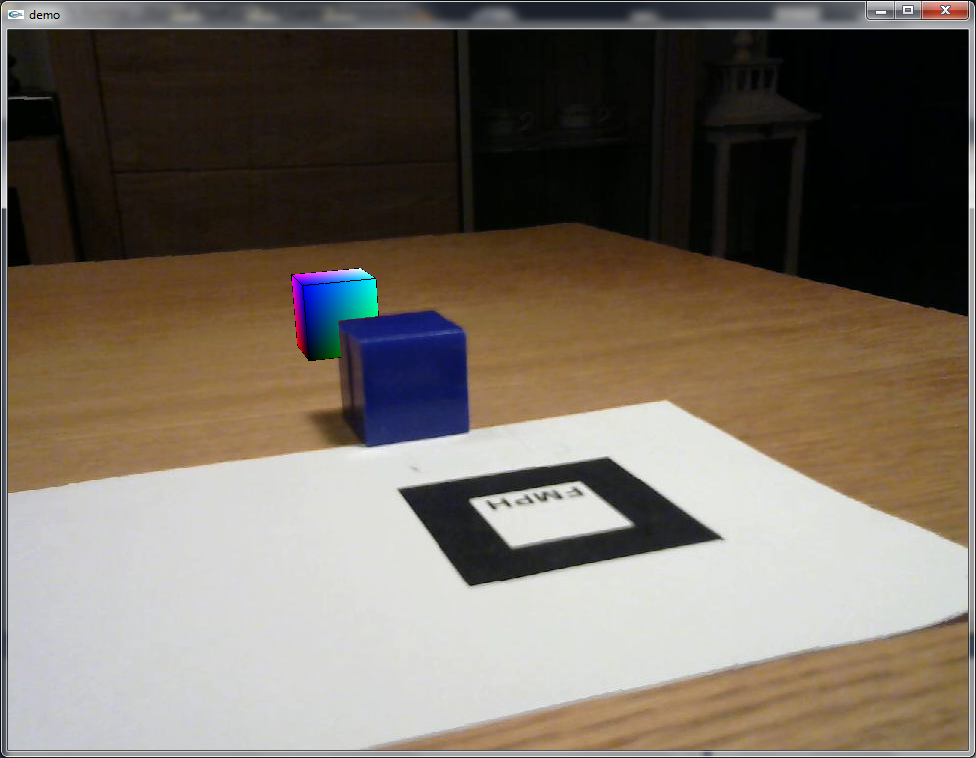
\includegraphics[max width=\textwidth]{pictures/screenshot-cubes.png}
 \caption{Jednoduchá ukážka oklúzie s kockami v našej aplikácii}
 \label{prototyp}
 \end{figure}

\section{3D modely}

Aby bolo možné vykresľovať 3D objekty na obrazovku, je potrebné ich reprezentovať v pamäti. Počas behu programu sa o to stará grafická knižnica, ale najjednoduchší spôsob ako do nej dáta naimportovať je uložiť ich do súboru.

Pre prácu s 3D modelmi existujú štandardizované formáty. Koncom deväťdesiatych rokov bol obľúbený formát VRML\footnote{Číta sa \emph{vermal}.}, ktorý je aj natívne podporovaný v ARToolkite, neskôr ho nahradil následník X3D \cite{Web3D}. Medzi dnes používanejšie formáty patrí napríklad COLLADA vyvíjaná združením Khronos Group \cite{Collada}, jej výhodou je vysoká kompatibilita s väčšinou nástrojov na modelovanie aj hernými enginmi. Iným obľúbeným formátom je STL (\emph{stereolithography}) používaný najmä na inžinierske účely ako je automatické projektovanie (po anglicky \emph{computer-aided design}, alebo \emph{CAD}) a~3D tlač. Výhodou je možnosť ukladania do textových aj binárnych súborov.

Zrejme najpoužívanejším 3D formátom je dnes Wavefront OBJ vyvinutý už neexistujúcou firmou Wavefront Technologies. OBJ je jednoduchý otvorený formát, ktorý sme sa rozhodli použiť.

\subsection{Formát Wavefront OBJ}

OBJ sme si vybrali, pretože sa jednoducho spracováva (\emph{parsuje}) a zároveň je všeobecne používaný a kompatibilný.

Formát vie zaznamenávať vrcholy (\emph{vertexy}), ich normály, textúrne súradnice a steny. Steny sú reprezentované n-uholníkmi danými zoznamami už definovaných vrcholov. Tieto vrcholy sú v zoznamoch uvedené v poradí v smere hodinových ručičiek \cite{Wavefront}.

Na ukážke \ref{dodecahedron} je zapísaný jednoduchý dvanásťsten vo formáte OBJ.

\lstset{ %
  backgroundcolor=\color{myyellow},
  breakatwhitespace=false,         % sets if automatic breaks should only happen at whitespace
  breaklines=true,                 % sets automatic line breaking
  commentstyle=\color{dkgreen},    % comment style
  keepspaces=true,                 % keeps spaces in text, useful for keeping indentation of code (possibly needs columns=flexible)
  keywordstyle=\color{blue},       % keyword style
  language=Python,                 % the language of the code
  otherkeywords={v, f},            % if you want to add more keywords to the set
  numbers=left,                    % where to put the line-numbers; possible values are (none, left, right)
  numbersep=5pt,                   % how far the line-numbers are from the code
  numberstyle=\tiny\color{gray}, % the style that is used for the line-numbers
  stepnumber=2,                    % the step between two line-numbers. If it's 1, each line will be numbered
  stringstyle=\color{mauve},     % string literal style
  tabsize=2,                       % sets default tabsize to 2 spaces
  title={dodecahedron.obj},                   % show the filename of files included with \lstinputlisting; also try caption instead of title
  caption={Dvanásťsten uložený vo formáte OBJ}
}

\begin{lstlisting}[label={dodecahedron}]
# Dodecahedron
v  -0.57735  -0.57735  0.57735
v  0.934172  0.356822  0
v  0.934172  -0.356822  0
v  -0.934172  0.356822  0
v  -0.934172  -0.356822  0
v  0  0.934172  0.356822
v  0  0.934172  -0.356822
v  0.356822  0  -0.934172
v  -0.356822  0  -0.934172
v  0  -0.934172  -0.356822
v  0  -0.934172  0.356822
v  0.356822  0  0.934172
v  -0.356822  0  0.934172
v  0.57735  0.57735  -0.57735
v  0.57735  0.57735  0.57735
v  -0.57735  0.57735  -0.57735
v  -0.57735  0.57735  0.57735
v  0.57735  -0.57735  -0.57735
v  0.57735  -0.57735  0.57735
v  -0.57735  -0.57735  -0.57735
f  19  3  2
f  12  19  2
f  15  12  2
f  8  14  2
f  18  8  2
f  3  18  2
f  20  5  4
f  9  20  4
f  16  9  4
f  13  17  4
f  1  13  4
f  5  1  4
f  7  16  4
f  6  7  4
f  17  6  4
f  6  15  2
f  7  6  2
f  14  7  2
f  10  18  3
f  11  10  3
f  19  11  3
f  11  1  5
f  10  11  5
f  20  10  5
f  20  9  8
f  10  20  8
f  18  10  8
f  9  16  7
f  8  9  7
f  14  8  7
f  12  15  6
f  13  12  6
f  17  13  6
f  13  1  11
f  12  13  11
f  19  12  11
\end{lstlisting}

Riadky začínajúce mriežkou slúžia na komentáre. Riadok začínajúci znakom \emph{v}~reprezentuje vrchol a obsahuje tri súradnice\footnote{Môže obsahovať štyri homogénne súradnice}. Riadky začínajúce znakmi \emph{vt} obsahujú textúrne súradnice zaznačené dvomi, či tromi číslami. Riadky začínajúce sa na~\emph{vn}~obsahujú normály vrcholov uložené tromi číslami.

Steny sú uložené na riadkoch začínajúcich znakom \emph{f}, po ktorom nasleduje zoznam vrcholov. Tieto vrcholy sú označené číslami, ktoré sa odvolávajú na poradie, v ktorom boli predtým definované. Steny môžu v svojich vrcholoch uchovávať aj textúrne súradnice, prípadne normály vrcholov. Tieto ďalšie informácie sa značia tak, že za poradové číslo vrcholu napíšeme lomku a pridáme poradové číslo predtým definovaných textúrnych súradníc. Za ďalšiu lomku môžeme zaznačiť poradové číslo normály. Pokiaľ je potrebné zaznamenať iba vrcholy a ich normály, vložia sa medzi ne dve lomky~\cite{Wavefront}.

Aby sme si ušetrili starosti pri spracovávaní a vykresľovaní modelu, rozhodli sme sa ho reprezentovať trojuholníkovou sieťou (po anglicky \emph{triangulated geometry}). To znamená, že každá stena je rozložená na steny ktoré majú len tri vrcholy. To má tú výhodu, že tieto trojuholníky sa dajú neskôr jednoducho vykreslovať pomocou OpenGL.

Na trianguláciu modelov sme použili otvorený modelovací nástroj Blender, ktorý dokáže exportovať modely do formátu OBJ v tejto podobe. OBJ príklad z ukážky \ref{dodecahedron} bol vytvorený týmto spôsobom.

Takto pripravený súbor načítame, spracujeme a vrcholy, normály a steny si uložíme do polí, z ktorých ich cez OpenGL rasterizujeme (ukážka na obrázku \ref{dodecahedron-render}).

\begin{figure}[h]
 \centering
 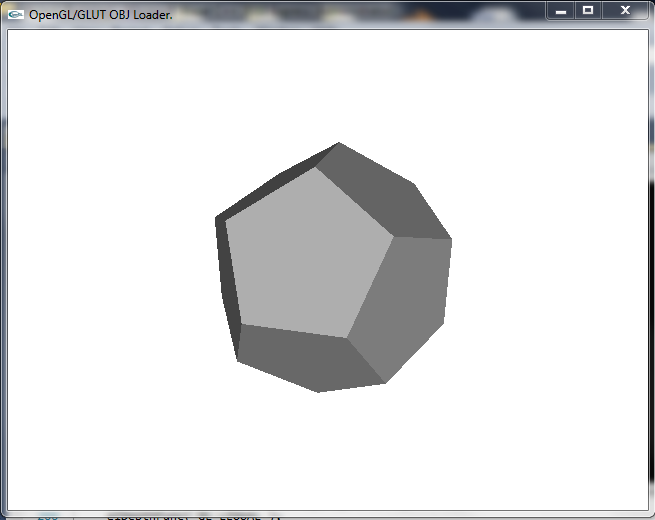
\includegraphics[max width=\textwidth]{pictures/screenshot-object-loader.png}
 \caption{Dvanásťsten načítaný zo súboru OBJ a vykreslený na obrazovku}
 \label{dodecahedron-render}
 \end{figure}

\section{Registrácia scény}

Na registráciu scény sme sa rozhodli použiť slobodnú knižnicu ARToolkit. Vznikla už v roku 1999 \cite{ARToolKit-b}, ale stále sa používa pre svoju jednoduchú rozšíriteľnosť. ARToolkit deteguje markery spôsobom popísaným v predchádzajúcej kapitole a nájde nám transformáciu, ktorou zarovnáme virtuálnu scénu v počítači do reálnej scény z~kamery.

Do tejto virtuálnej scény môžeme pomocou OpenGL vykresľovať to, čo potrebujeme. V prípade, že vieme aké bude osvetlenie fyzickej scény, môžeme podľa toho nastaviť osvetlenie vo virtuálnej scéne, aby neskutočné objekty pôsobili skutočnejšie.

Marker, ktorý používame na registráciu je priložený v prílohe A tejto práce. Na obrázku \ref{sova-marker} je ukážka modelu vykresleného na marker.

\begin{figure}[h]
 \centering
 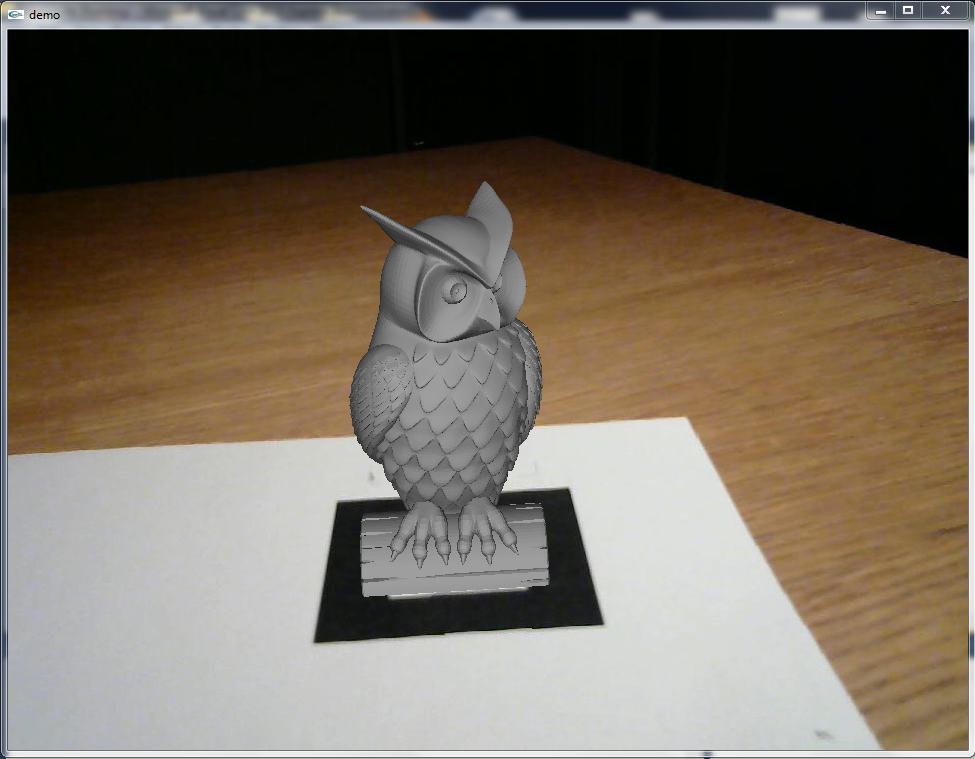
\includegraphics[max width=\textwidth]{pictures/screenshot-object.png}
 \caption{Model sovy vykreslený a umiestnený na marker v našej demo aplikácii}
 \label{sova-marker}
 \end{figure}

\section{Kalibrácia kamery}

Pokiaľ vytvárame aplikáciu s rozšírenou realitou dosiahnutou pomocou počítačového videnia a potrebujeme, aby zobrazovala virtuálne objekty čo najpresnejšie, je potrebné nakalibrovať kameru.

Kamery sa líšia kus od kusu a preto je potrebné vykonať meranie, ktorým získame parametre konkrétneho zariadenia. Tieto parametre potom zohľadníme pri rozpoznávaní obrazu.

V prípade bežnej dierkovej kamery (po anglicky \emph{pinhole camera}) sa tieto parametre usporiadavajú do matice parametrov kamery (\emph{camera matrix}), ktorá je vynásobením matice vnútorných (\emph{intrinsic}) parametrov s vonkajšími (\emph{extrinsic}) parametrami, ktoré udávajú transformáciu 3D súradníc svetu na 3D súradnice kamery. Určenie matice vnútorných parametrov kamery sa nazýva kalibrácia kamery.

\[
 A=
  \begin{pmatrix}
    \alpha_{x} & \gamma     & u_{0}\\
    0          & \alpha_{y} & v_{0}\\
    0          & 0          & 1
  \end{pmatrix}
\]

Matica vnútorných parametrov obsahuje parametre, ktoré sa dajú vypočítať nasledovne.

\begin{align}
\alpha_{x} = f \cdot m_{x} \\
\alpha_{y} = f \cdot m_{y}
\end{align}

Kde $m_{x}$ a $m_{y}$ sú škálovacie faktory pixelov a $f$ je ohnisková vzdialenosť. $\gamma$ je skresľovací koeficient medzi osami $x$ a $y$ a obvykle ho môžeme nastaviť na 0. $u_{0}$ a $v_{0}$ označujú posunutie optického stredu\footnote{Optický stred je bod, ktorý je prienikom optickej osi s priemetňou.} (po anglicky \emph{principal point}) v oboch osiach \cite{Hartley03}.

Tieto parametre je možné (pokiaľ sú známe vonkajšie parametre kamery) vypočítať z minimálne jednej fotky kalibračného vzoru\footnote{Obvykle sa pre zvýšenie presnosti použijú výsledky z viacerých fotiek vytvorených z rôznych uhlov. My sme ich pri kalibrácií vyhotovili dvadsať.}. Vhodné je fotiť napríklad šachovnicu alebo pole kruhov. Od začiatku merania nesmie kamera opticky preostrovať, ani meniť ohniskovú vzdialenosť (približovať), pretože by sa parametre zmenili.

Po transformácii maticou parametrov kamery vieme zvrátiť deformáciu obrazu.

\[
z_{c}\begin{bmatrix}
u\\
v\\
1\end{bmatrix}=A \begin{bmatrix}
R & T\end{bmatrix}\begin{bmatrix}
x_{w}\\
y_{w}\\
z_{w}\\
1\end{bmatrix}
\]

Pre kalibráciu kamery sme použili jednoduchý program využívajúci knižnicu pre~počítačové videnie OpenCV (obrázok \ref{kalib}). Táto knižnica implementuje šikovné metódy na detekciu kalibračnej siete aj výpočet parametrov z nameraných údajov. Taktiež umožňuje výpočet šošovkového skreslenia spôsobeného použitím bežnej kamery so šošovkou.

\begin{figure}[h]
 \centering
 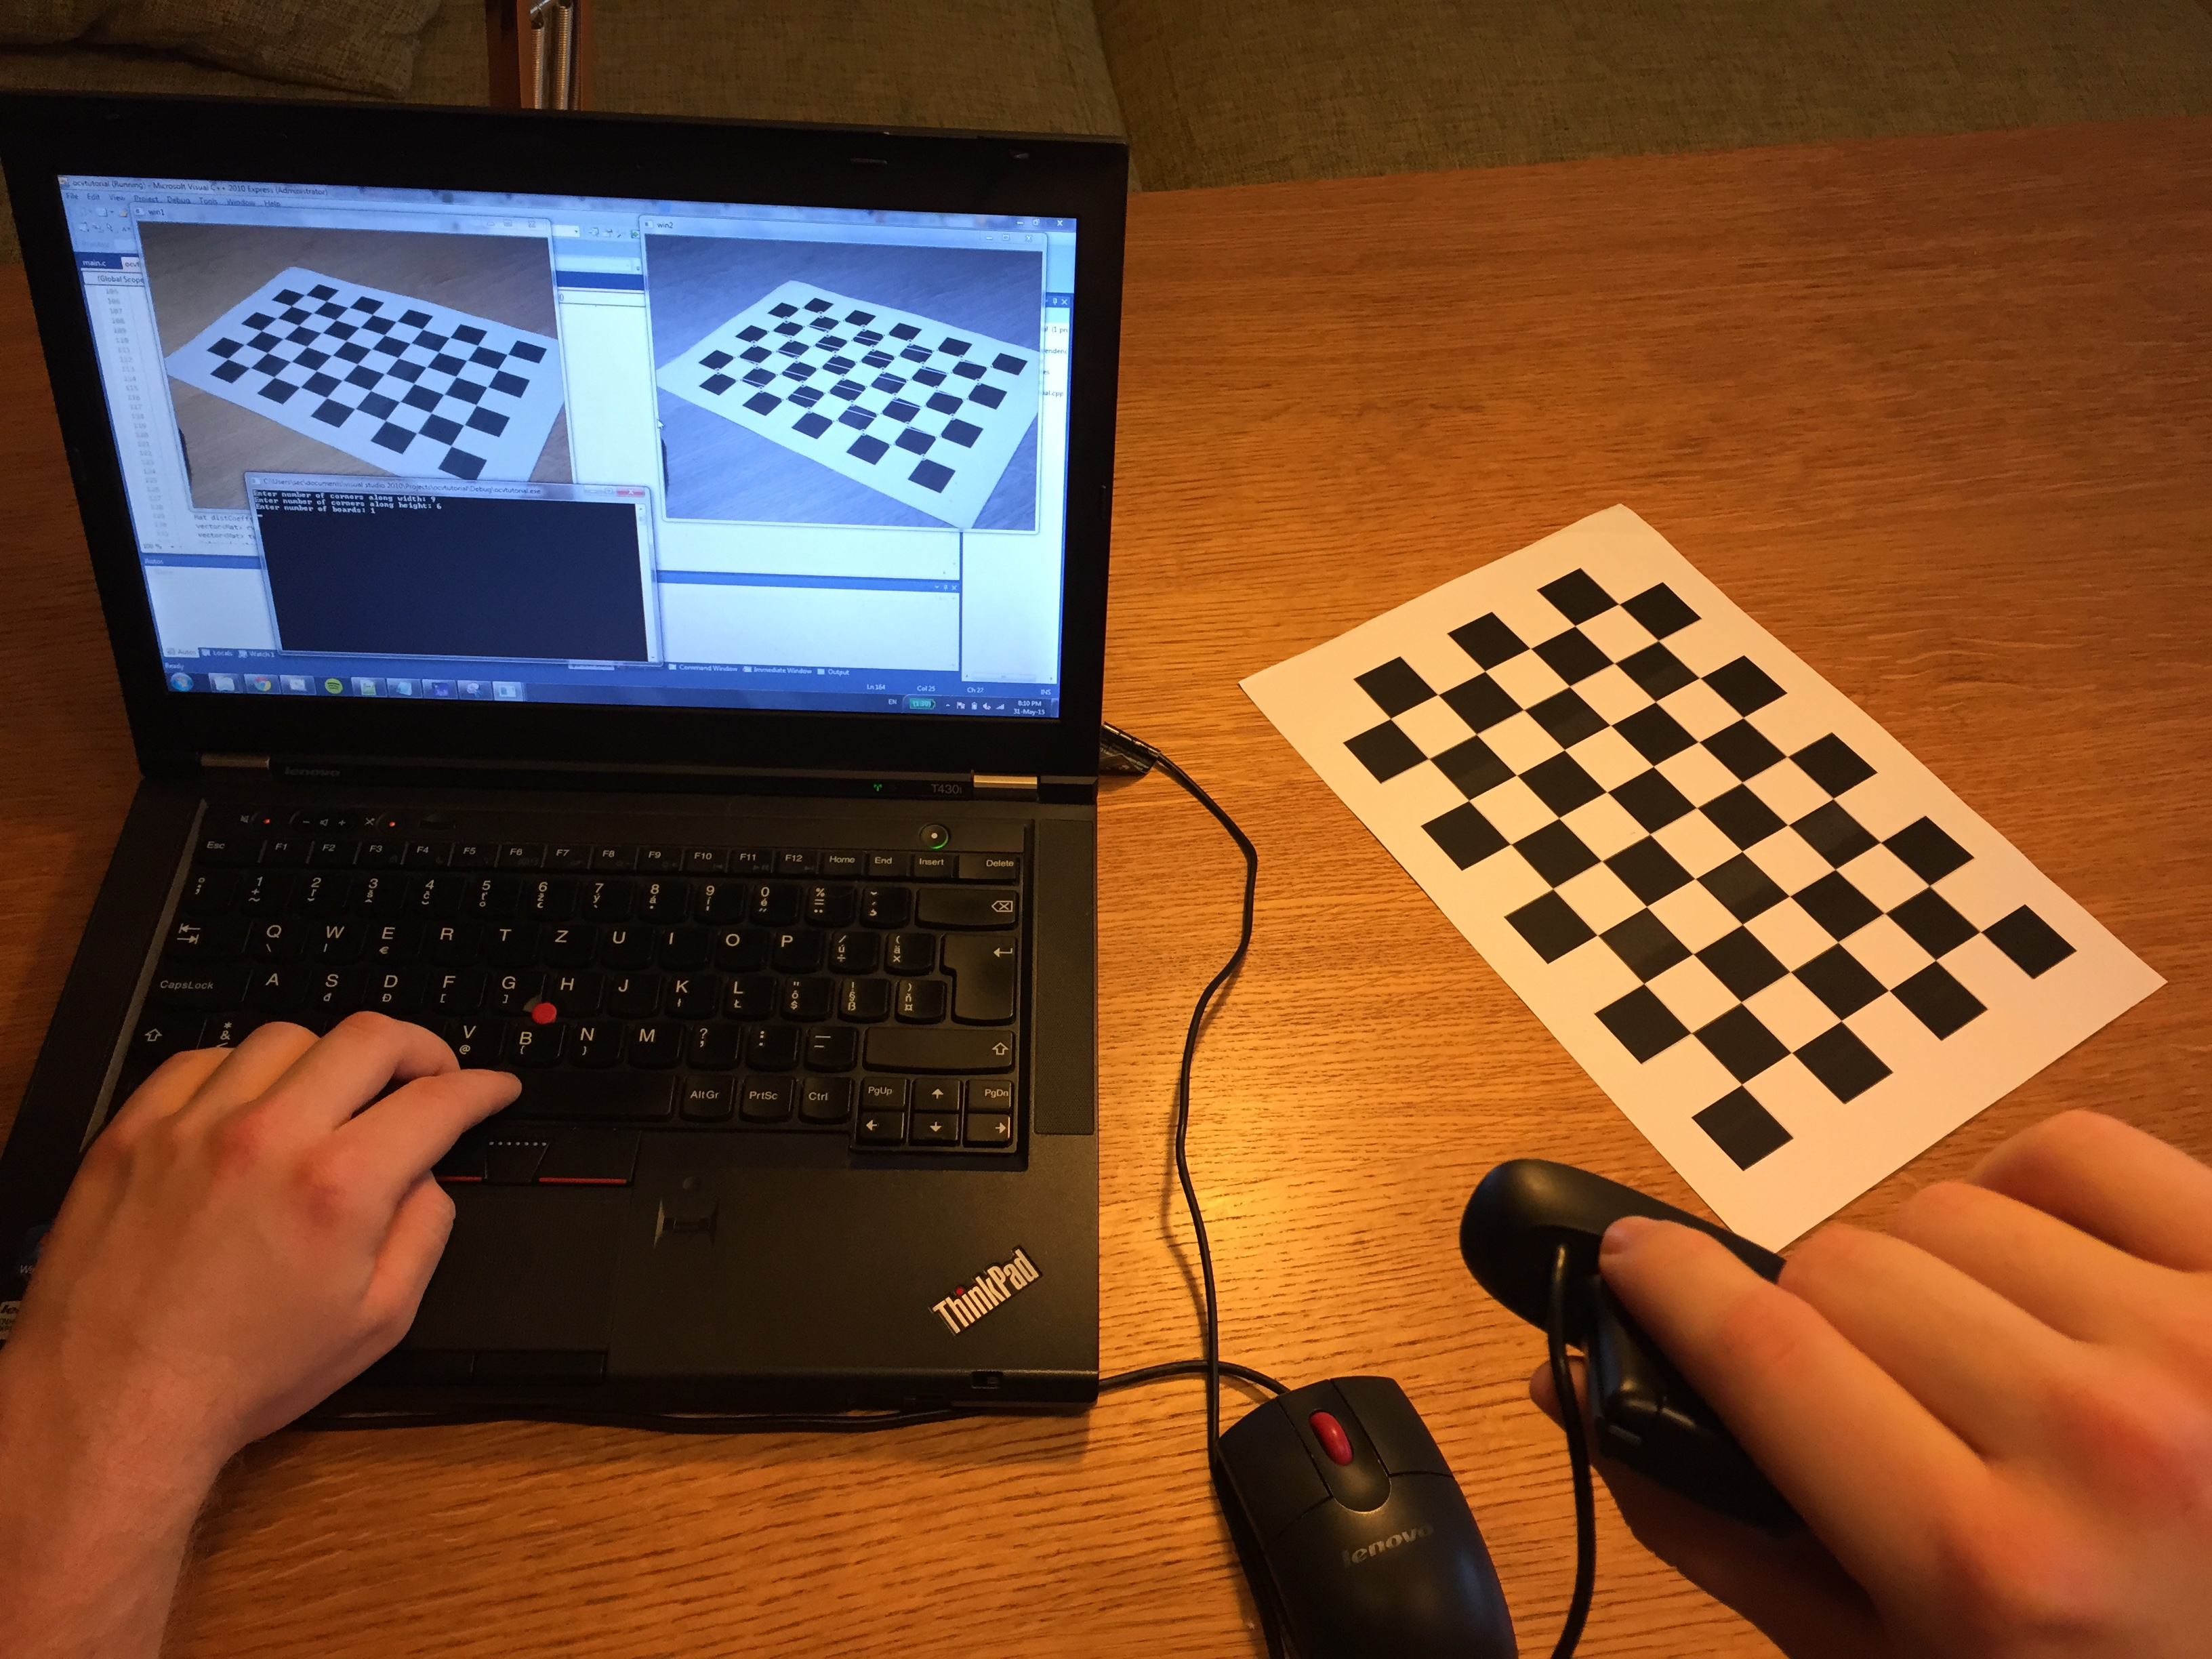
\includegraphics[max width=\textwidth]{pictures/kalibracia-foto.jpg}
 \caption{Kalibrácia kamery}
 \label{kalib}
 \end{figure}

\section{Príprava oklúderu}

Predtým ako môžeme implementovať oklúziu, potrebujeme mať vybraný oklúder a jeho digitálnu 3D reprezentáciu. Zvolili sme si na to viacero postupov.

\subsection{Modelovanie}

Najzákladnejší spôsob ako získať 3D model skutočného objektu, je ho jednoducho odmerať a vymodelovať v modelovacom programe. Pri prvom prototype ukázanom v článku \ref{section-prototyp} sme aplikovali zjednodušený postup a zvolili si za oklúder kocku, pretože má len osem vrcholov na jednoducho vymenovateľných súradniciach. Rozhodli sme sa vynechať načítavanie modelu a kocku popísať priamo v programe (znázornené na ukážke~\ref{kocka}). Vďaka tomu, že každé dve kocky sú si podobné stačí po popísaní kocky nájsť len správny škálovací koeficient.

\lstset{ %
  backgroundcolor=\color{myyellow},
  breakatwhitespace=false,         % sets if automatic breaks should only happen at whitespace
  breaklines=true,                 % sets automatic line breaking
  commentstyle=\color{dkgreen},    % comment style
  keepspaces=true,                 % keeps spaces in text, useful for keeping indentation of code (possibly needs columns=flexible)
  keywordstyle=\color{blue},       % keyword style
  language=C,                 % the language of the code
  otherkeywords={GL_GREATER, GL_KEEP, GL_STENCIL_TEST, GL_REPLACE, GL_ALWAYS, GLfloat},            % if you want to add more keywords to the set
  numbers=left,                    % where to put the line-numbers; possible values are (none, left, right)
  numbersep=5pt,                   % how far the line-numbers are from the code
  numberstyle=\tiny\color{gray}, % the style that is used for the line-numbers
  stepnumber=2,                    % the step between two line-numbers. If it's 1, each line will be numbered
  stringstyle=\color{mauve},     % string literal style
  tabsize=2,                       % sets default tabsize to 2 spaces
  caption={Reprezentácia kocky},                   % show the filename of files included with \lstinputlisting; also try caption instead of title
}

\begin{lstlisting}[label={kocka}]
	const GLfloat cube_vertices [8][3] = {
	{1.0, 1.0, 1.0}, {1.0, -1.0, 1.0}, {-1.0, -1.0, 1.0}, {-1.0, 1.0, 1.0},
	{1.0, 1.0, -1.0}, {1.0, -1.0, -1.0}, {-1.0, -1.0, -1.0}, {-1.0, 1.0, -1.0} };
	const short cube_faces [6][4] = {
	{3, 2, 1, 0}, {2, 3, 7, 6}, {0, 1, 5, 4}, {3, 0, 4, 7}, {1, 2, 6, 5}, {4, 5, 6, 7} };
\end{lstlisting}

\subsection{3D skener SMISS}

SMISS, teda \emph{Scalable Multifunctional Indoor Scanning System} je zariadenie vyvinuté na \emph{Fakulte matematiky, fyziky a informatiky Univerzity Komenského}, ktoré dokáže skenovať trojrozmerné objekty \cite{Kovacovsky13}. Objekt, ktorý je potrebné nasnímať sa položí na otočný stôl. Na tento stôl je pod uhlom namierená kamera a projektor. Projektor premieta na snímaný objekt štruktúrované svetlo. Toto svetlo projektuje pruhy, ktorými „rozreže“ skenovaný objekt na jednotlivé roviny, pričom každá rovina je osvetlená a zakódovaná iným vzorom svetla. Každé nasvietenie je odfotené kamerou. Na začiatku skenovania je objekt rozdelený iba na zopár rovín, tie sa ale postupne delia na tenšie rezy, čím vzniká vyššia detailnosť. Keď sú nasnímané všetky požadované nasvietenia, motor stôl pootočí a projektor začne objekt znovu nasvecovať z nového uhlu \cite{Kovacovsky12-a, Kovacovsky12-b}.

Počítač z obrazu dekóduje jednotlivé roviny a po zosnímaní zo všetkých strán vytvorí mračno bodov (po anglicky \emph{point cloud}) reprezentujúce objekt. Na výsledné mračno bodov môžeme aplikovať trianguláciu a tým získame polygonálny model, ktorý môžeme použiť ako oklúder. Priemerná prestnosť SMISSu je \SI{500}{\micro\metre} \cite{Kovacovsky12-b}.

Na skeneri sme skenovali lepiacu pásku, ktorá je na obrázku \ref{paska} a výsledok jej skenovania je na obrázku \ref{paska-cloud}.

\begin{figure}[h]
 \centering
 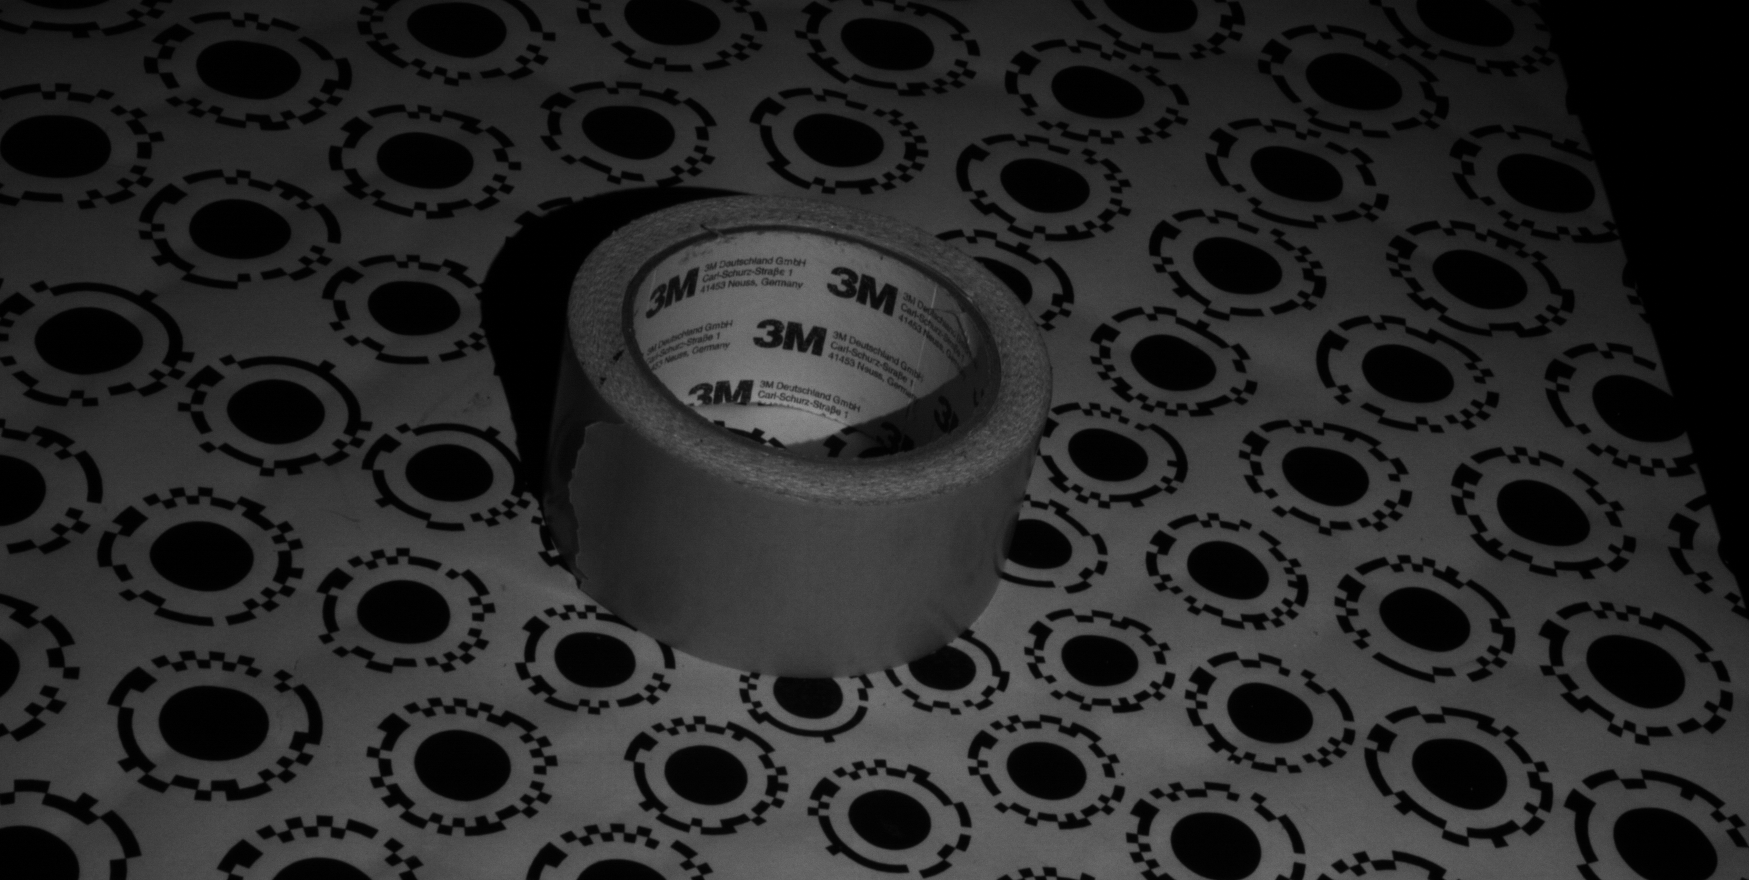
\includegraphics[max width=\textwidth]{pictures/smiss.png}
 \caption{Lepiaca páska z pohľadu skeneru SMISS}
 \label{paska}
 \end{figure}

\begin{figure}[h]
 \centering
 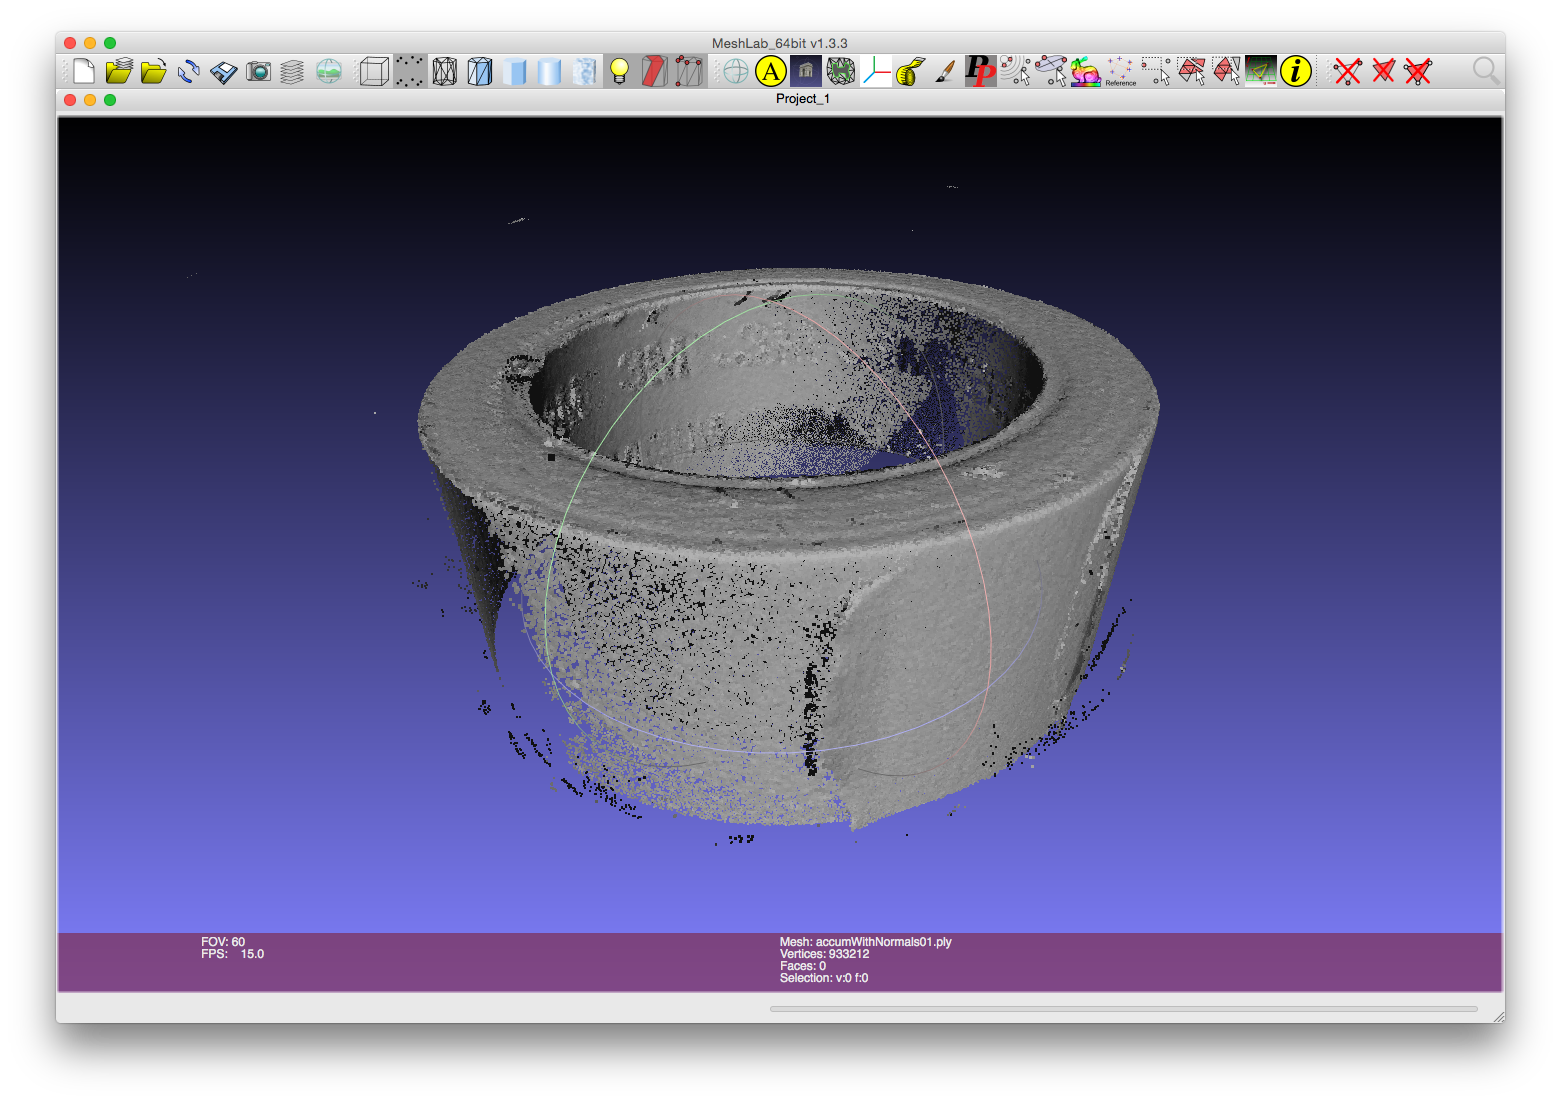
\includegraphics[max width=\textwidth]{pictures/smiss-pointcloud.png}
 \caption{Mračno bodov, ktoré je výstupom skenovania SMISSom}
 \label{paska-cloud}
 \end{figure}

\subsection{3D tlač}

Druhou možnosťou, ako získať oklúder a jeho virtuálny 3D model je namodelovať ho v~počítači a potom ho vytlačiť na 3D tlačiarni. Na vytvorenie takéhoto modelu je vhodný napríklad Blender, z ktorého ho potom môžeme vyexportovať do OBJ pre~aplikáciu aj STL pre tlač.

STL model nahráme do \emph{slicera}, to je program, ktorý zoberie model a ‚rozreže‘ ho na~veľký počet 2D vrstiev. Príkladom je slicer MakerBot Desktop, dodávaný k~tlačiarňam značky MakerBot. Výška vrstvy závisí od nastaveného rozlíšenia. Tieto dáta sa potom vložia do tlačiarne a tá začne roztápať plastovú náplň (\emph{fillament}) a~nanášať ju vrstvu po vrstve na seba.

Inteligentný slicer dokáže do dutého modelu dorobiť sieť vnútorných stien, aby sa nerozpadol. V prípade, že tlačený predmet obsahuje časti, ktoré prevísajú von a teda by ich nebolo ako tlačiť do vzduchu, môže slicer dopočítať podpery, ktoré sa vytlačia spolu s modelom a po vytlačení sa odrežú. V prípade použitia tlačiarne s dvomi tlačiacimi hlavami je dokonca možné použiť dva fillamenty, z toho jeden vodou rozpustný, ktorým sa tlačia podpery. Po tlači sa model len ponorí do vody.

Dnešné 3D tlačiarne zvládajú rozlíšenie okolo \SI{100}{\micro\metre}, čo je okolo 255 dpi, teda 255 vrstiev na jeden palec výšky. Nevýhodou je, že s kvalitou rýchlo narastá aj čas, ktorý tlačenie potrvá.

Na tlačiarni sme tlačili model sovy z obrázku \ref{sova-blend} a jej výtlačok je na obrázku \ref{sova-print}.

\begin{figure}[h]
 \centering
 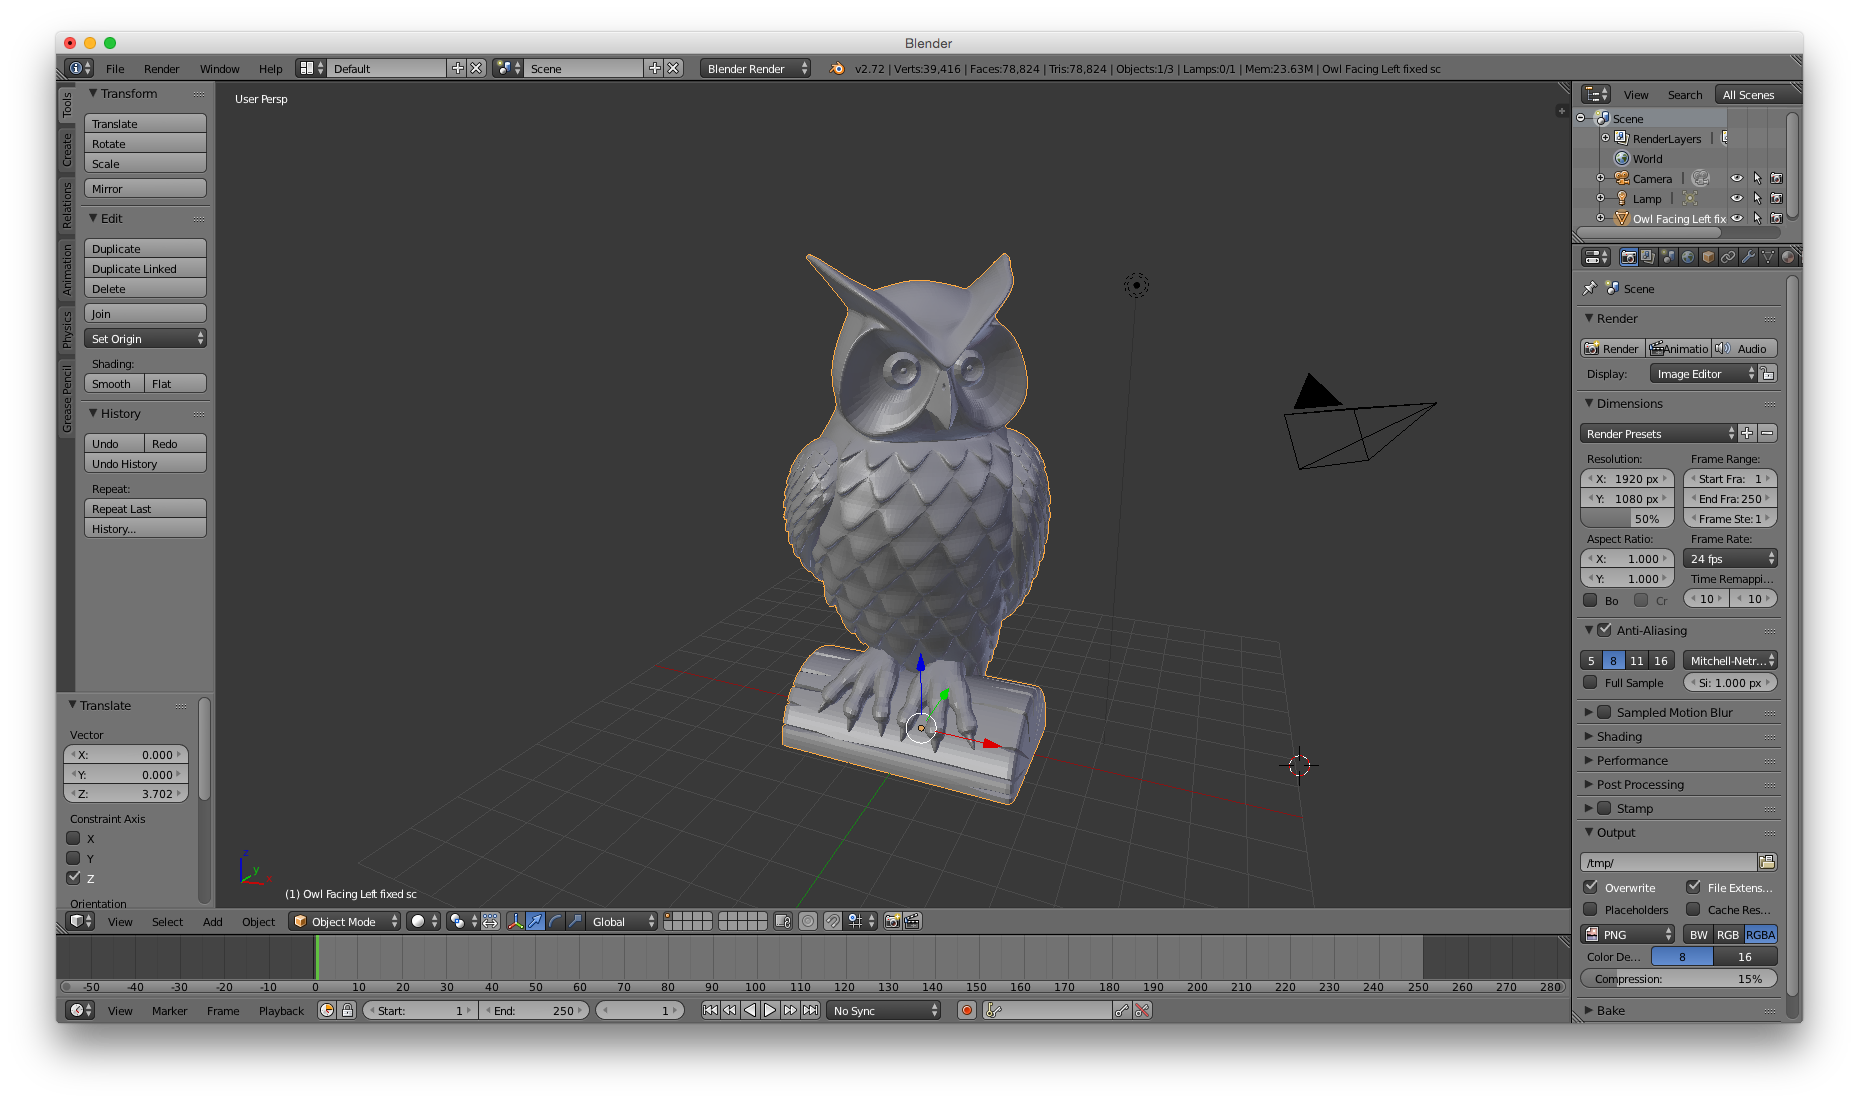
\includegraphics[max width=\textwidth]{pictures/owl-blender.png}
 \caption{Digitálny model sovy, otvorený v modelovacom programe Blender. Autorom modelu je modelár Tom Cushwa \cite{Cushwa}}
 \label{sova-blend}
 \end{figure}

\begin{figure}[h]
 \centering
 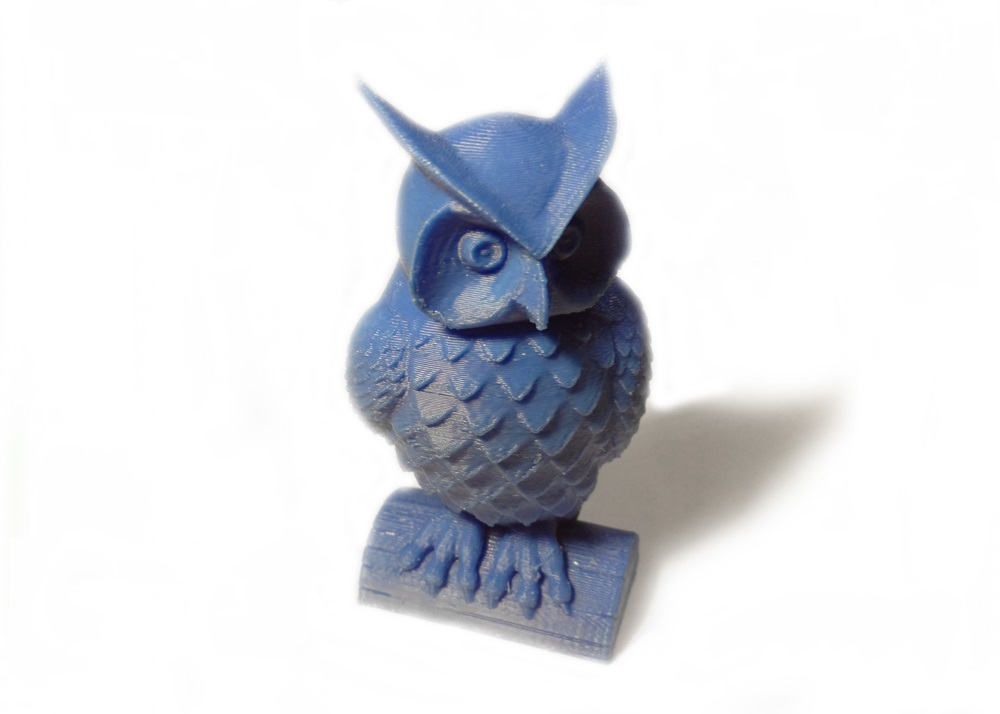
\includegraphics[max width=\textwidth]{pictures/owl-model.jpg}
 \caption{Fyzický model sovy, ktorý sme vytlačili na 3D tlačiarni}
 \label{sova-print}
 \end{figure}

\section{Oklúzia v rozšírenej realite}

Ak chceme v rozšírenej realite zobrazovať virtuálne objekty tak, aby ich úplne, alebo čiastočne prekrývali fyzické objekty na scéne, je potrebné, aby pre každý tento fyzický objekt aplikácia okrem virtuálneho 3D modelu poznala aj jeho veľkosť a polohu na~scéne voči markeru, prípadne ho vedela inak rozoznať.

Program následne objekty, prípadne ich časti, ktoré sú prekryté oklúderom ne\-vy\-kres\-lí a rovnako ne\-vy\-kres\-lí ani samotný oklúder. Na mieste, kde majú byť objekty prekryté sa teda zobrazí stopa z videa, ktorá je na pozadí. Táto stopa na danom mieste obsahuje pôvodný fyzický objekt zosnímaný kamerou a tým sa vytvorí ilúzia, že virtuálne objekty sú prekryté tými reálnymi. Pri oklúzií je obzvlášť dôležité mať správne nakalibrovanú kameru, aby sa virtuálne objekty premietali čo najpresnejšie na~svoje miesta.

Najprv si vykreslíme pomocou OpenGL oklúder do \emph{stencil bufferu}. Tento buffer je binárnym obrázkom veľkosti vykresľovaného okna a slúži ako úložné miesto na dočasné informácie o danom obraze. Na každý bod v stencil bufferi zapíšeme true, pokiaľ by sa na dané súradnice v normálnom pohľade vykreslila časť oklúdera. Neskôr pri~vykresľovaní virtuálnych objektov, ktoré sa majú nachádzať za oklúderom, robíme pre~každý pixel jednoduchú kontrolu. Nachádza sa na týchto súradniciach v stencil bufferi hodnota true? Ak sa nachádza, tak pixel nevykreslíme, pretože nemá byť vidieť a~pokračujeme ďalej. Táto logika je znázornená na ukážke \ref{okluzia-kod}.

\lstset{ %
  backgroundcolor=\color{myyellow},
  breakatwhitespace=false,         % sets if automatic breaks should only happen at whitespace
  breaklines=true,                 % sets automatic line breaking
  commentstyle=\color{dkgreen},    % comment style
  keepspaces=true,                 % keeps spaces in text, useful for keeping indentation of code (possibly needs columns=flexible)
  keywordstyle=\color{blue},       % keyword style
  language=C,                 % the language of the code
  otherkeywords={GL_GREATER, GL_KEEP, GL_STENCIL_TEST, GL_REPLACE, GL_ALWAYS, GLfloat},            % if you want to add more keywords to the set
  numbers=left,                    % where to put the line-numbers; possible values are (none, left, right)
  numbersep=5pt,                   % how far the line-numbers are from the code
  numberstyle=\tiny\color{gray}, % the style that is used for the line-numbers
  stepnumber=2,                    % the step between two line-numbers. If it's 1, each line will be numbered
  stringstyle=\color{mauve},     % string literal style
  tabsize=2,                       % sets default tabsize to 2 spaces
  caption={Implementácia oklúzie},                   % show the filename of files included with \lstinputlisting; also try caption instead of title
}

\begin{lstlisting}[label={okluzia-kod}]
//render occluder to stencil buffer
glEnable(GL_STENCIL_TEST);
glStencilOp(GL_REPLACE, GL_REPLACE, GL_REPLACE);
glStencilFunc(GL_ALWAYS, 1, 0xffffffff);
DrawOccluder();

//render occluded object
glStencilFunc(GL_GREATER, 1, 0xffffffff);
glStencilOp(GL_KEEP, GL_KEEP, GL_KEEP);
DrawObject();
glDisable(GL_STENCIL_TEST);
\end{lstlisting}

\section{Výsledky}

Aplikácia má funkcionalitu, ktorú sme si špecifikovali. Na obrázku \ref{scene} je znázornený príklad scény na ktorej predvádzame aplikáciu. Na obrázku \ref{no-occlusion} je snímka obrazovky z aplikácie v situácií, kedy registrujeme scénu, ale oklúder neprekrýva vykreslovaný objekt\footnote{Autorom voľne šíriteľného modelu stromu v pozadí je theswiss z portálu Thingiverse \cite{theswiss14}.} a k oklúzií preto nedochádza.

\begin{figure}[h]
 \centering
 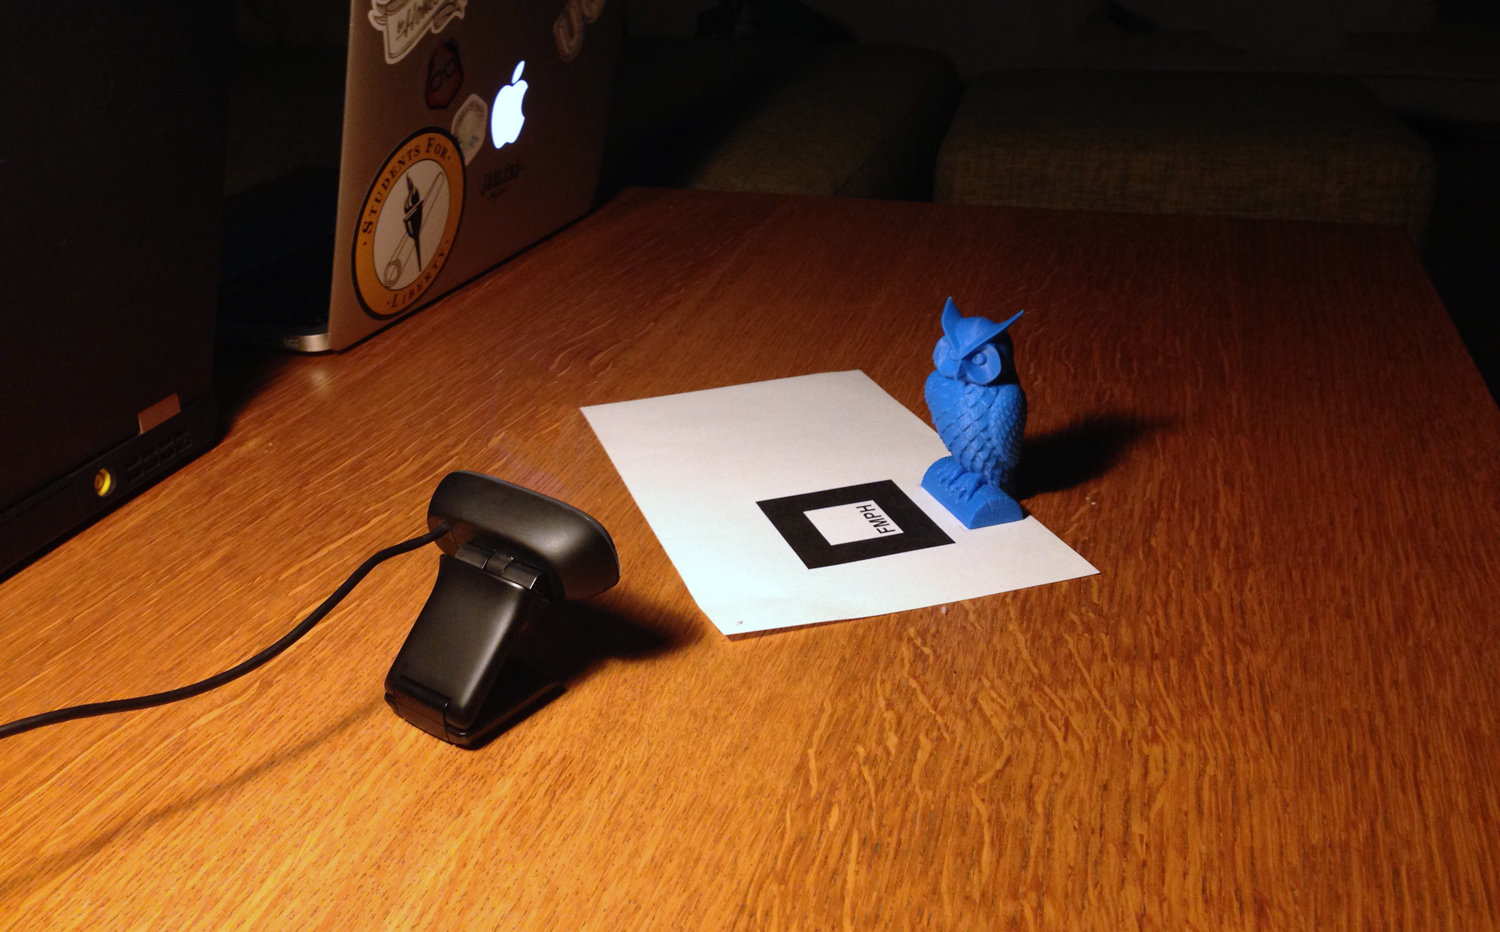
\includegraphics[max width=\textwidth]{pictures/scene.jpg}
 \caption{Scéna na ktorej demonštrujeme oklúziu. Modrý model sovy je oklúderom.}
 \label{scene}
 \end{figure}

\begin{figure}[h]
 \centering
 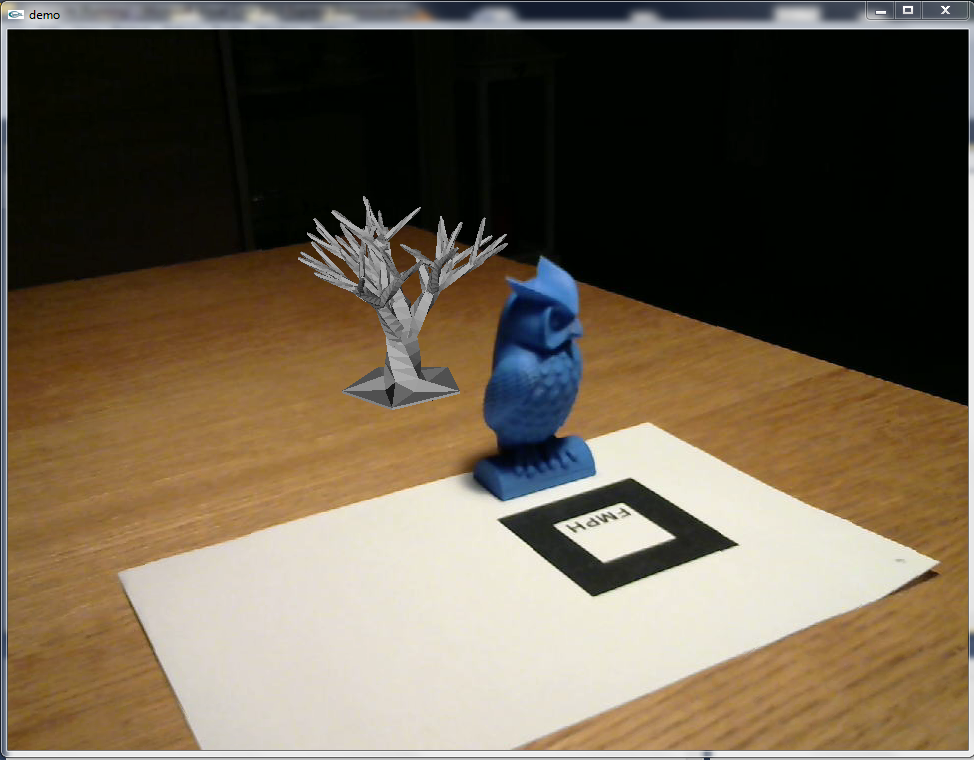
\includegraphics[max width=\textwidth]{pictures/screenshot-separate.png}
 \caption{Skutočný a virtuálny objekt sa neprekrývajú, takže k oklúzii nedochádza}
 \label{no-occlusion}
 \end{figure}

Aby sme sa uistili, že máme fyzický oklúder položený na správnu relatívnu pozíciu voči markeru, môžeme si v aplikácii zapnúť vykresľovanie oklúderu a pozrieť sa, nakoľko presne sa prekrývajú (znázornené na obrázku \ref{show-occluder}).

Ak je oklúder správne zarovnaný a vypneme jeho vykresľovanie na obrazovku, dosiahneme oklúziu, ako je vidno na obrázku \ref{true-occlusion}.

\begin{figure}[h]
 \centering
 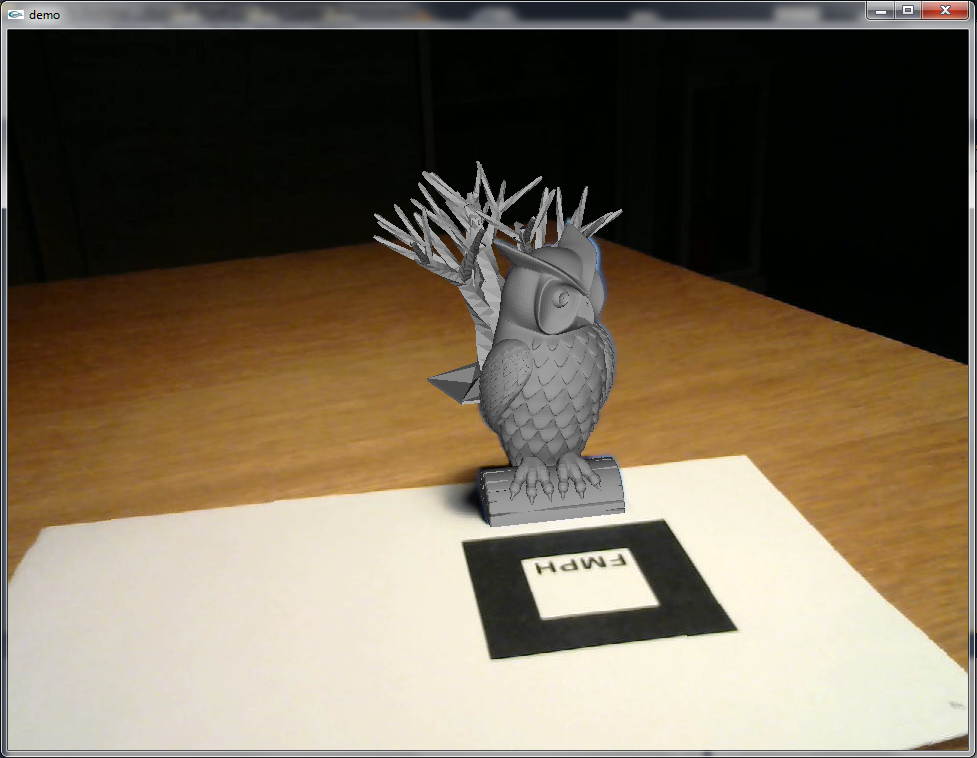
\includegraphics[max width=\textwidth]{pictures/screenshot-occluder.png}
 \caption{Natočili sme scénu tak, aby sa objekty prekrývali a nechali sme vykreslovať aj virtuálny model oklúderu, ktorý sa pomocou markeru registruje cez skutočnú sovu.}
 \label{show-occluder}
 \end{figure}

\begin{figure}[h]
 \centering
 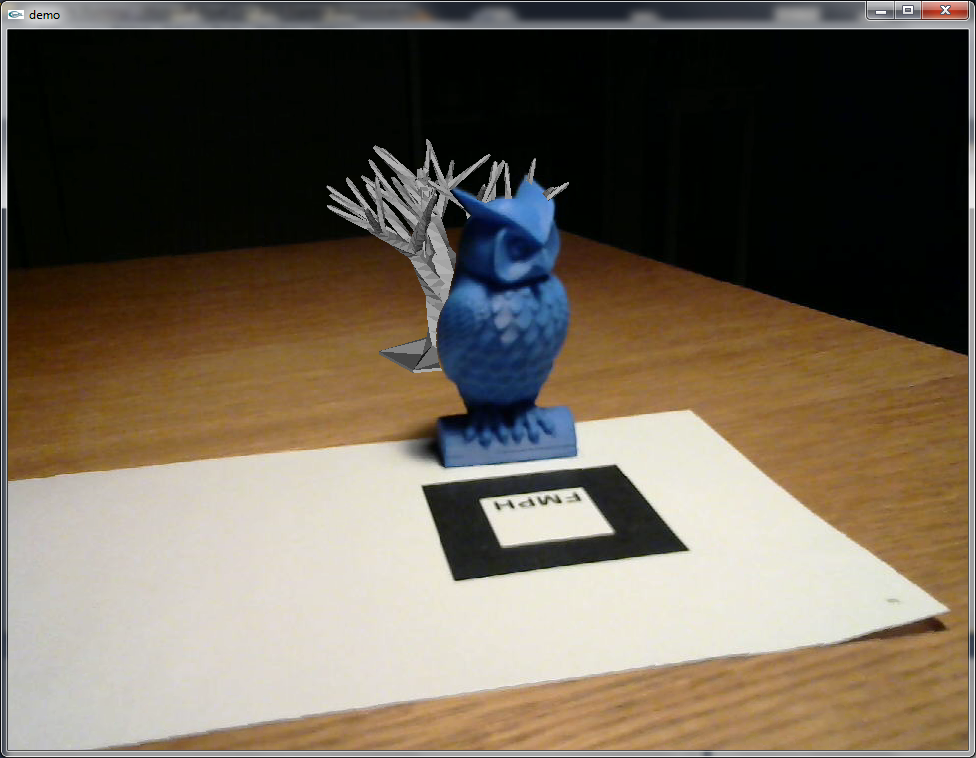
\includegraphics[max width=\textwidth]{pictures/screenshot-occlusion.png}
 \caption{V predchádzajúcej scéne sme nechali oklúder vykresľovať iba do stencil bufferu a výsledkom je oklúzia s fyzickým objektom.}
 \label{true-occlusion}
 \end{figure}
 
 \subsection{Výkon aplikácie}
 
 Bez ohľadu na zložitosť (počet vrcholov) skúšaných modelov nám aplikácia bežala na našom hardvéri plynulo pri framerate 29 až 30 snímkov za sekundu (\emph{framerate} vyjadruje rýchlosť obnovovania obrazovky). Informácie o použitých modeloch sú uvedené v tabuľke 4.1. Na obrázku \ref{benchmark} sú vykreslené všetky modely naraz, tiež pri framerate 30 snímkov za sekundu.
  
 Hodnota 30 snímkov za sekundu je limitovaná našou kamerou, ktorá nezvláda robiť snímky rýchlejšie a aplikácia teda musí po spracovaní snímku čakať na nasledovný snímok.
 
 Aplikáciu sme spúšťali na počítači s procesorom Intel Core i3 taktovaným na 2.4 GHz, 8 GB pamäte a integrovanou grafickou kartou Intel HD 3000. Snímky z kamery boli spracovávané v rozlíšení 960 na 720 pixelov.
 
 \begin{center}
   \begin{tabular}{| l | r | r |}
     \hline
     model &  počet vrcholov &  počet stien \\ \hline\hline
     sova (oklúder) & 39416 & 7824 \\ \hline
     loď Enterprise & 2680 & 5372 \\ \hline
     drak Alduin & 8160 & 16074 \\ \hline
     mesto Atlantis & 41437 & 83190 \\ \hline \hline
     spolu & 91693 & 112460 \\ \hline
   \end{tabular}
   \captionof{table}{Údaje o modeloch použitých pri testovaní výkonu aplikácie} 
 \end{center}
 
\begin{figure}[h]
 \centering
 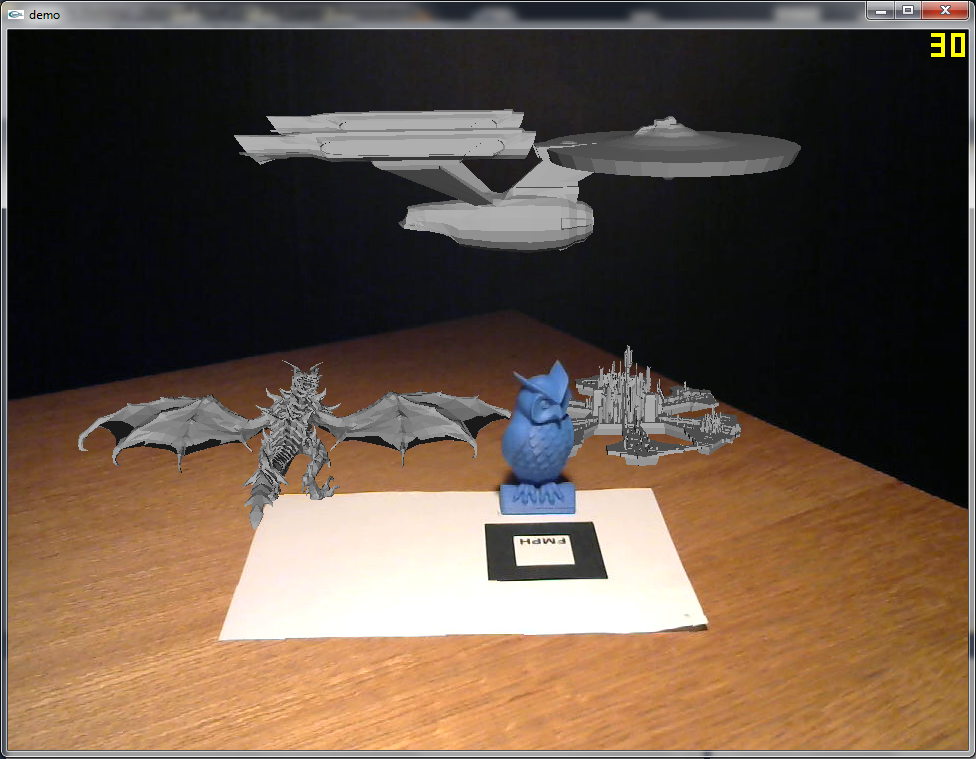
\includegraphics[max width=\textwidth]{pictures/benchmark.png}
 \caption{Vykresľovanie viacerých modelov naraz}
 \label{benchmark}
 \end{figure}
 
 \subsection{Možné problémy a nepresnosti}
 
 Detekcia markeru funguje spoľahlivo a aplikácia obvykle nemá problémy s identifikáciou scény pokiaľ je celý marker viditeľný. Zaznamenali sme iba jeden prípad kedy detekcia zlyhá a to keď je časť markeru v tieni. Táto situácia môže ľahko nastať, pokiaľ je scéna nasvietená ostrým svetlom (napríklad stolnou lampou) spoza oklúderu a oklúder zatieňuje časť markeru.
 
 Problémy s nepresnosťou oklúzie môžu nastať niekoľkými spôsobmi, prípadne ich kombináciou. Fyzický model oklúderu je potrebné relatívne umiestniť voči markeru veľmi presne, čo môže byť obtiažne. Nepresnosť taktiež môže spôsobiť nesprávne naškálovaný virtuálny model oklúderu. Nenakalibrovaná, alebo nedostatočne presne nakalibrovaná kamera spôsobuje ďaľšiu nepresnosť. Tieto nepresnosti sa prejavujú tak, že výrez vo vykresľovanom objekte je posunutý oproti fyzickému oklúderu a nie je s~ním presne zarovnaný.